\section{ADCS Threat Model and Systematic Blind Spots}
\label{sec:threat_model}

We consider an attacker with an ordinary domain foothold and the template-modification or enrollment rights required by the tested condition. The defender can collect directory, CA and KDC records but may receive incomplete or delayed fields. Correct raw issuance and authentication records are trust assumptions; optional CA exports have a separately declared fault budget. The experiments concern controlled issuance and use, not the entire ADCS attack taxonomy.

\subsection{Heterogeneous Access Control Multigraph Formalization}
We model an enterprise Active Directory forest and its integrated Public Key Infrastructure as a directed heterogeneous multigraph (Figure~\ref{fig:adcs_schema}).

\begin{definition}[Identity Multigraph Schema]
\label{def:identity_schema}
Let $\mathcal{G} = (\mathcal{V}, \mathcal{E}, \phi, \psi)$ be a directed heterogeneous multigraph, where:
\begin{itemize}
    \item $\mathcal{V}$ is the finite set of identity and PKI vertices, and $\phi: \mathcal{V} \to \mathcal{T}_V$ is a node-type assignment function mapping vertices to the entity set:
    \begin{equation}
\fitmath{\begin{gathered}\mathcal{T}_V = \{\text{User}, \text{Group}, \text{Computer},\\  \text{CertificateTemplate}, \text{EnterpriseCA}, \text{Domain}\}\end{gathered}}
\end{equation}
    \item $\mathcal{E}$ is the finite set of directed edges, and $\psi: \mathcal{E} \to \mathcal{T}_E$ maps edges to relationship types:
    \begin{equation}
\fitmath{\begin{gathered}\mathcal{T}_E = \{\text{MemberOf}, \text{GenericAll},\text{GenericWrite},\\
    \text{WriteOwner},\text{WriteDacl},\text{Enroll},\\
    \text{ExtendedRight},\text{EnablesEnrollment},\\
    \text{IssuedBy},\text{TrustedForNTAuth}\}\end{gathered}}
\end{equation}
    \item Each node $v \in \mathcal{V}$ is associated with a raw feature vector $\mathbf{x}_v \in \mathbb{R}^{d_{\phi(v)}}$. For certificate templates $t \in \mathcal{V}_{\text{Template}}$, $\mathbf{x}_t \in \{0, 1\}^{10}$ encodes security configuration flags, including whether the template permits enrollee-supplied SANs (\texttt{CT\_FLAG\_ENROLLEE\_SUPPLIES\_SUBJECT}), requires manager approval (\texttt{CT\_FLAG\_PEND\_ALL\_REQUESTS}), or specifies Client Authentication EKUs (\texttt{1.3.6.1.5.5.7.3.2}).
\end{itemize}
\end{definition}

An attack path $p$ from an initial compromised user foothold $u_{\text{attacker}} \in \mathcal{V}_{\text{User}}$ to a high-value domain target $v_{\text{target}} \in \mathcal{V}_{\text{Domain}}$ is a sequence of alternating vertices and edges:
\begin{equation}
\fitmath{\begin{gathered}p = (v_0, e_1, v_1, e_2, \dots, e_k, v_k),\\ v_0 = u_{\text{attacker}}, \quad v_k = v_{\text{target}}\end{gathered}}
\end{equation}
In an ADCS privilege escalation, the path traverses intermediate membership and ACL delegation edges to a certificate template $t$, leverages an enterprise CA $c$ to issue an administrative credential, and culminates in a domain-level credential takeover.

\begin{figure}[t]
\centering
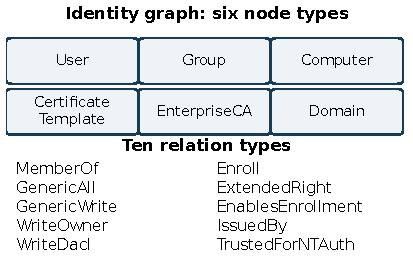
\includegraphics[width=\linewidth]{figures/revised_identity_schema.pdf}
\caption{Identity-graph abstraction: six node classes and ten relation types, matching Definition~\ref{def:identity_schema}. Relation instances depend on the directory export; not every type is exercised by every experiment.}
\label{fig:adcs_schema}
\end{figure}

\paragraph{Evaluated attack scope}
The live interventions test enrollee-supplied-subject policy and certificate mapping, with template mutation and restoration. These are ESC1-style issuance conditions with an ESC4-style modification step~\cite{schroeder2021certified}. Some archived filenames refer to other ESC scenarios, but those names do not establish successful exploitation. The synthetic learning predicate assumes resolved enrollment permissions; it does not validate ESC1--ESC15 coverage. CA-administration compromise, relay, issuance-policy group links and later ESC variants require separate policy and protocol evidence. They are outside the live coverage claim.

\subsection{Template Rollback and Snapshot Evidence}
Directory extraction tools such as BloodHound, SharpHound and Certipy provide configuration snapshots. Their scheduling is deployment-specific. Under temporal mutation-and-rollback attacks (such as ESC4 and ESC9), an attacker exploits transient write permissions to mutate a template, obtain a rogue certificate, and immediately roll back the attributes to their original configuration.

\begin{definition}[Static Snapshot Invariance under Rollback]
Let $t_0 < t_1 < t_2 < t_3$ denote the sequence of discrete timestamps in an attack execution lifecycle:
\begin{itemize}
    \item $t_0$: Pristine baseline state of directory $\mathcal{G}_{t_0}$.
    \item $t_1$: The attacker executes an LDAP modification adding \texttt{Enroll} permissions or setting \texttt{CT\_FLAG\_ENROLLEE\_SUPPLIES\_SUBJECT} on template $t$, yielding state $\mathcal{G}_{t_1}$.
    \item $t_2$: The attacker submits a certificate request and receives an issued certificate $\text{Cert}_{\text{admin}}$ valid for 1 year.
    \item $t_3$: The attacker rolls back the template modifications, restoring the directory attributes to their baseline state, yielding $\mathcal{G}_{t_3}$.
\end{itemize}
\end{definition}

\paragraph{Snapshot Indistinguishability and Evidence Scope}
For a projection restricted to configuration attributes restored by rollback, let $h_0$ and $h_1$ denote the digests before and during the mutation. The relevant equality is:
\begin{equation}
\fitmath{\begin{gathered}\text{SHA-256}(\mathcal{G}_{t_0}) = h_0\end{gathered}}
\end{equation}
\begin{equation}
\fitmath{\begin{gathered}\text{SHA-256}(\mathcal{G}_{t_1}) = h_1\end{gathered}}
\end{equation}
\begin{equation}
\fitmath{\begin{gathered}\text{SHA-256}(\mathcal{G}_{t_3}) = h_0\end{gathered}}
\end{equation}

This is a conditional indistinguishability argument for that projection, not evidence that the entire AD database is bit-identical. A detector restricted to this projection cannot distinguish the restored sequence from an unchanged configuration with the same projection. This is a statement about information available to the detector, not an empirical zero-recall estimate. The certificate can remain usable subject to validity, revocation, trust and account mapping. It does not imply that every directory or audit artifact disappears.

\subsection{Protocol Discontinuity: PKCS\#10 ASN.1 SAN Concealment and CA--KDC Logging Gap}
Collecting both CA and KDC Security events does not necessarily supply a shared certificate key. The relevant gap is missing certificate identity in the captured issuance event, rather than disjoint event-field names.

\paragraph{Captured event projections}
The selected issuance fields in Listing~\ref{lst:ca_event} are
\[\fitmath{\pi_{\mathrm{CA}}=\{\mathrm{RequestId},\mathrm{Requester},\mathrm{Subject},\mathrm{Attributes}\}.}\]
The certificate-bearing successful KDC record additionally exposes
\[\fitmath{\begin{gathered}
\pi_{\mathrm{KDC}}=\{\mathrm{TargetUserName},\mathrm{PreAuthType},\\
\mathrm{CertIssuerName},\mathrm{CertSerialNumber},\mathrm{CertThumbprint}\}.
\end{gathered}}\]
Neither Disposition nor SKID is shown in the selected 4887 payload. SKID and the other certificate identifiers used by the contract are obtained from the CA database export when available. Different field names alone say nothing about whether a join is possible: the issue is whether the captured values supply a shared, issuer-scoped certificate identity.

\paragraph{SAN fields in requests and audit records}
When an attacker requests a certificate with a rogue Subject Alternative Name (e.g., impersonating the Domain Administrator), the SAN attribute can be supplied through two distinct mechanisms:
\begin{enumerate}
    \item \textbf{Explicit RPC Attribute String:} Passed via the \texttt{Attributes} string parameter of \texttt{ICertRequest::Submit} (e.g., \texttt{"SAN:upn=Administrator@domain.local"}). In this configuration, the CA security log explicitly populates the \texttt{Attributes} field in Event ID 4887.
    \item \textbf{Raw PKCS\#10 ASN.1 Binary Extension:} Embedded directly within the cryptographic Certificate Signing Request (CSR) under the \texttt{szOID\_SUBJECT\_ALT\_NAME2} (\texttt{2.5.29.17}) extension attribute.
\end{enumerate}

Our forensic investigation of live archived GOAD event streams reveals that when an attacker employs the PKCS\#10 ASN.1 CSR extension (as executed natively by modern exploit tooling), the CA event log omits the SAN string entirely from the XML event payload:
\begin{lstlisting}[language=XML,caption={Selected fields from the independent 2019 enabled-condition capture: Security record 20539. The raw XML is retained in the artifact.},label=lst:ca_event]
<Event xmlns="http://schemas.microsoft.com/win/2004/08/events/event">
  <System>
    <Provider Name="Microsoft-Windows-Security-Auditing"/>
    <EventID>4887</EventID>
    <TimeCreated SystemTime="2026-11-10T10:53:51.393283900Z"/>
    <EventRecordID>20539</EventRecordID>
  </System>
  <EventData>
    <Data Name="RequestId">7</Data>
    <Data Name="Requester">Q1LAB\q1.enroller</Data>
    <Data Name="Subject">CN=q1.enroller</Data>
    <Data Name="Attributes">
CertificateTemplate:Q1Evidence
ccm:WIN-NA2FC16NO63.q1lab.test</Data>
  </EventData>
</Event>
\end{lstlisting}

Listing~\ref{lst:ca_event} contains a template and client-machine attribute, but no textual SAN UPN. The issued public certificate does contain the requested administrative SAN, and an exact-certificate successful KDC event independently checks its use. A query requiring a textual administrative SAN in this issuance event has no such input here; this is a concrete missing-field case, not a measured universal SIEM false-negative rate. The selected issuance event supplies a Request ID, whereas the certificate-bearing KDC record supplies issuer, serial, and thumbprint. SKID is optional CA-database enrichment, not a field demonstrated by this listing. The CA database export supplies the issuer-scoped bridge evaluated in Section~\ref{sec:evaluation}.
